\documentclass[UTF8,a4paper,12pt]{ctexart}
\usepackage[left=2.54cm, right=2.54cm, top=3.18cm, bottom=3.18cm]{geometry}
% -- text font --
% compile using Xelatex
%\setmainfont{Microsoft YaHei}	% 微软雅黑
%\setmainfont{YouYuan}	% 幼圆	
%\setmainfont{NSimSun}	% 新宋体
%\setmainfont{KaiTi}	% 楷体
%\setmainfont{SimSun}	% 宋体
%\setmainfont{SimHei}	% 黑体

\usepackage{times}
%\usepackage{mathpazo}
%\usepackage{fourier}
%\usepackage{charter}
%\usepackage{helvet}

\usepackage{amsmath, amsfonts, amssymb}	% math equations, symbols
\usepackage[english]{babel}
\usepackage{color}		% color content
\usepackage{graphicx}	% import figures
\usepackage{url}		% hyperlinks
\usepackage{bm}			% bold type for equations
\usepackage{hyperref}	% bookmarks
\hypersetup{bookmarks, unicode, colorlinks}	% unicode

\newtheorem{myDef}{Definition}
\numberwithin{equation}{section}
\numberwithin{figure}{section}
\numberwithin{table}{section}
\renewcommand{\bold}[1]{~$\bm{#1}$~}

\title{神经网络的联合学习猜想}
\author{ 匿名1 \thanks{学号: 11531015, e-mail: xueshengke@zju.edu.cn},匿名2 \thanks{学号: 11531016, e-mail: 1042430841@qq.com} }
\date{2016~年~6~月~18~日}

\begin{document}
	\maketitle
\begin{abstract}
目前,神经网络的训练方法仅是最小化一个目标函数,比如最小化平方误差项,通过梯度下降方法更新网络中的可学习的参数,即权值和偏置。然而,在实验和理论的神经科学领域中,已经发现了一种的突触内在可塑性的性质~(有时也被称作信息最大化算法)~。它改变的是神经元的非线性,即激活函数本身。但是,该机制未被广泛引入人工神经网络的训练研究中。本文提出了一种基于信息最大化和平方误差项最小化结合的训练人工神经网络的方法——联合学习机制,的猜想。
\end{abstract}

\section{简介}
人工神经网络包含了非线性处理单元,设计用于处理复杂的非线性的、非平稳的信号处理问题。在监督学习问题中,我们提供了训练数据集包含输入\bold{x},和期望输出值\bold{d}。我们旨在找到输入与输出的映射关系,可以建模\bold{x}和\bold{d}之间的复杂函数关系。为了解决这样的问题,我们建立一个人工神经网络,通过合适的学习算法来推测隐含在训练数据中的关系。目前,大多数人工神经网络的学习算法是依赖于更新神经元之间的连接权值\bold{w}和偏置\bold{b}。通常的做法是最小化网络的实际输出\bold{y}和期望输出\bold{d}之间的均方误差~(关于所有的输入)~,其中误差定义为~$\bm{e}=\frac{1}{2}\parallel \bm{d} - \bm{y} \parallel^2$~。对于多层神经网络,我们运用误差反向传播算法,使网络中所有层的权值和偏置都能得到更新。多层网络中反向传播的步骤中,计算目标函数关于权值的梯度~$\partial \bm{e}/\partial \bm{w}$~不过是链式求导的规则的应用。关键思想是目标函数关于一个神经元的输入的梯度~$\partial \bm{e}/\partial \bm{u}^\ell$~可以使用后一层中对应神经元关于其输入的梯度~$\partial \bm{e}/\partial \bm{u}^{\ell+1}$~计算得到。反向传播可以遍历所有的神经元,从输出层神经元沿着权值连接往输入层传递。一旦这些梯度值~$\partial \bm{e}/\partial \bm{u}^\ell$~求得,目标函数关于权值的梯度~$\partial \bm{e}/\partial \bm{w}^\ell$~也就可以直接计算得出。

到目前为止,实验和理论的神经科学研究都普遍遵循~Hebb's~规则。它提出记忆是存储在突触权值中,而学习是一个改变突触权值的过程。不过最近的实验结果揭露了神经元能够改变内部的激励以适应输入的不同程度的改变。这种新颖的机制称作内在可塑性。它被假设是为了在保持一个独立神经元平均激活率的稳态,同时,最大化其信息容量~\cite{stemmler1999voltage}\cite{triesch2005gradient}\cite{triesch2007synergies}~。实际上,在忽视能量限制的前提下,内在可塑性规则非常接近~Bell~和~Sejnowski~的信息最大化算法~\cite{bell1995information}~。

\section{信息最大化算法} \label{section2}
在生物神经元中,内在可塑性将能量消耗考虑为一个重要的限制。但是这个限制对人工神经网络是不必要的,所以我们只考虑其最大化信息容量的特性。我们应用的信息最大化学习算法是~Bell~和~Sejnowski~\cite{bell1995information}~提出的。

一个神经网络的输出为\bold{Y}而输入为\bold{X}。最基本的问题如何最大化其互信息,定义为
\begin{align}
I(\bm{Y},\bm{X})=H(\bm{Y})-H(\bm{Y} \mid \bm{X}), \label{eq:I_Y_X}
\end{align}
其中~$H(\bm{Y})$~是输出的熵,而~$H(\bm{Y} \mid \bm{X})$~是输出的熵中不属于输入的部分。为了简化分析,式~\eqref{eq:I_Y_X}~中所有项可微,仅考虑网络中关于参数\bold{w}的梯度。将~\eqref{eq:I_Y_X}~关于\bold{w}求偏导,得到
\begin{align}
\frac{\partial}{\partial \bm{w}} I(\bm{Y},\bm{X})=\frac{\partial}{\partial \bm{w}} H(\bm{Y}).
\end{align}
因为~$H(\bm{Y} \mid \bm{X})$~与\bold{w}无关。于是,我们得到:最大化互信息~$I(\bm{Y},\bm{X})$~,等价于最大化输出输出熵~$H(\bm{Y})$~。

\paragraph{单输入单输出网络} 当我们传入一个输入~$x$~,经过一个激活函数~$h(x)$~(带有可调节参数~$w$~),得到一个输出~$y$~。则在~$x$~的概率密度函数的高密度部分对齐函数~$h(x)$~的最陡峭的部分时,互信息~$I(y,x)$~和~$H(y)$~被最大化。见图~\ref{fig:maximization}~。
\begin{figure}[htbp]
	\centering
	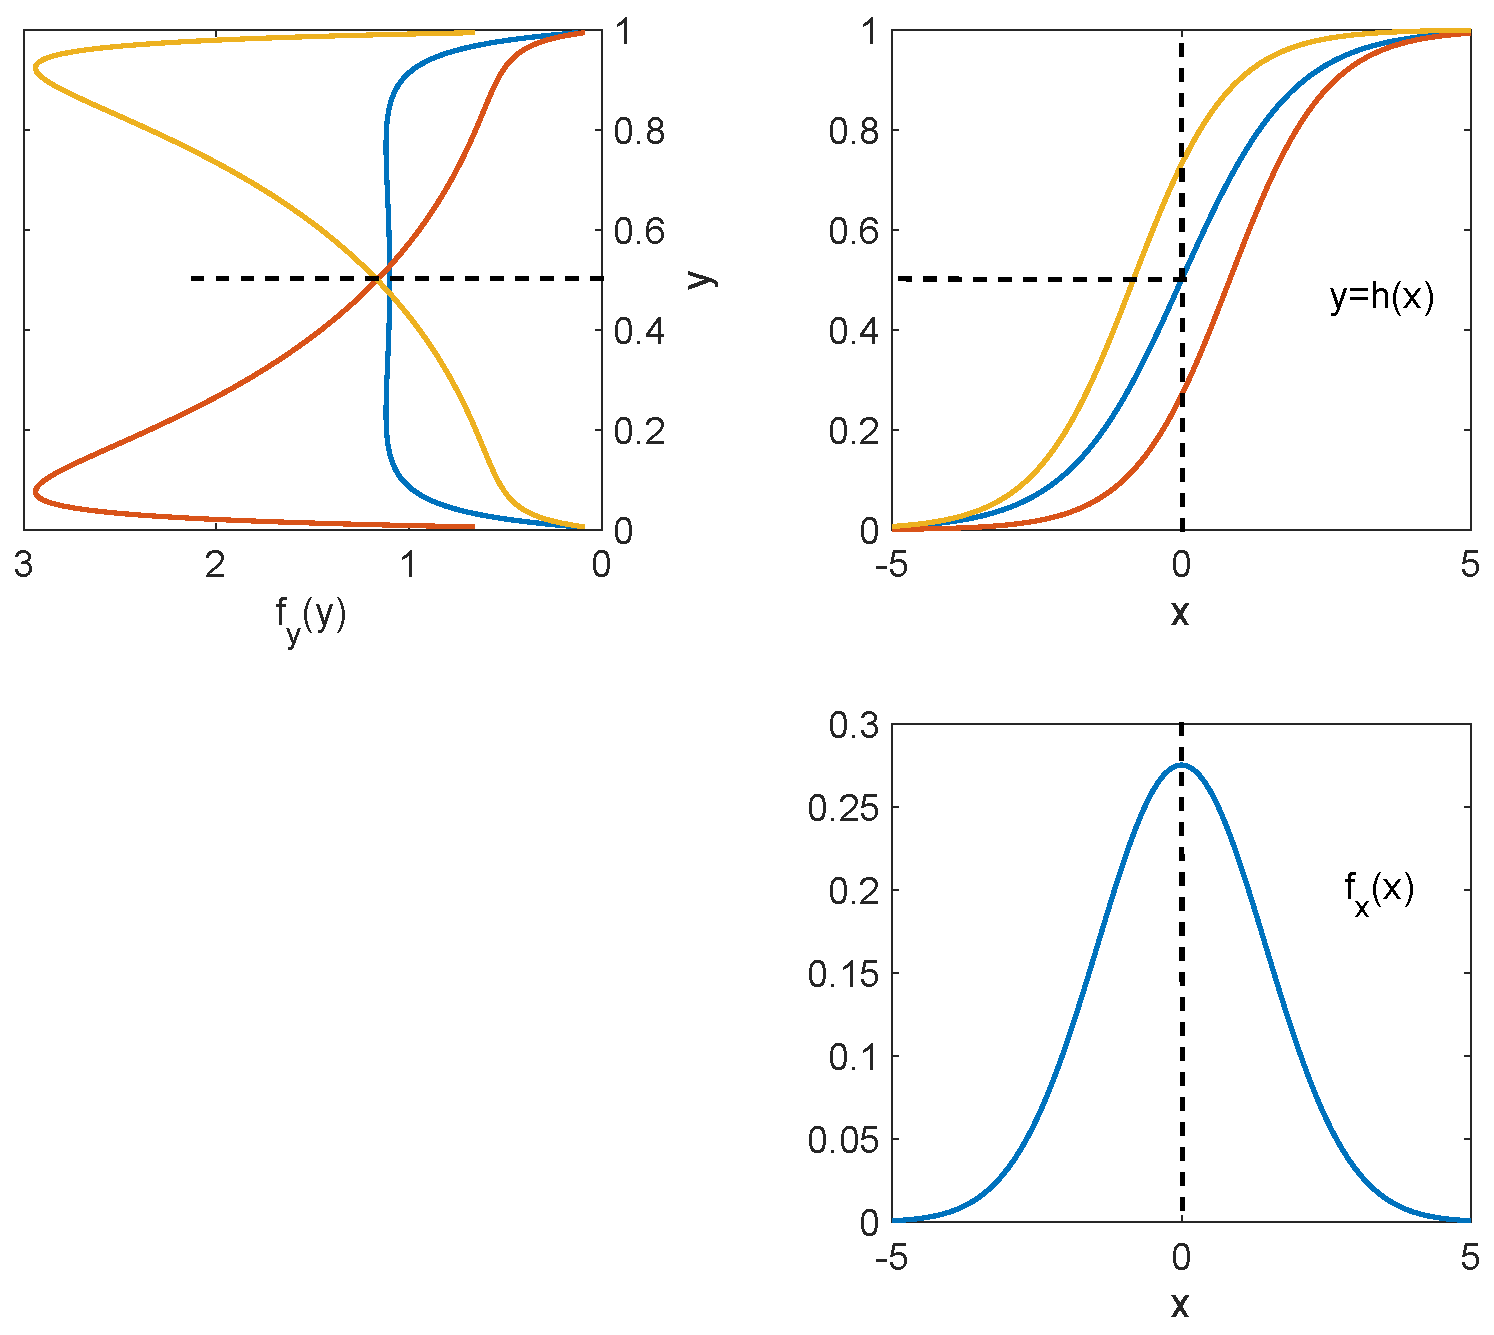
\includegraphics[width=0.6\textwidth]{maximization.pdf}
	\caption{输入~$x$~服从概率密度分布~$f_x(x)$~,图中为高斯分布,经过一个非线性的激活函数~$h(x)$~(由参数~$w$~调节),得到输出~$y$~的概率密度分布~$f_y(y)$~。}\label{fig:maximization}
\end{figure}

当~$h(x)$~是单调递增或递减时,输出的概率密度函数~$f_y(y)$~,可以用输入的概率密度函数~$f_x(x)$~表示~\cite{papoulis2002probability}~,
\begin{align}
f_y(y)=\frac{f_x(x)}{|\partial y / \partial x|}. \label{eq:f_y}
\end{align}
输出熵~$H(y)$~可以表示为,
\begin{align}
H(y)=-E[\ln f_y(y)]=-\int_{-\infty}^{\infty} f_y(y) \ln f_y(y)~dy, \label{eq:H_y}
\end{align}
其中~$E[\cdot]$~表示期望。把~\eqref{eq:f_y}~和~\eqref{eq:H_y}~代入,得到,
\begin{align}
H(y)=E\left[ \ln\left| \frac{\partial y}{\partial x} \right| \right] - E[\ln f_x(x)].
\end{align}
其中的右边第二项,即~$x$~的熵,可以认为不会因~$h(x)$~的参数~$w$~改变而影响。于是为了最大化~$y$~的熵,我们只需要关注右边的第一项,也就是输入对输出影响度的对数平均值。假设训练数据~$x$~近似分布~$f_x(x)$~,给出一种梯度上升学习规则~\cite{bell1995information}~,
\begin{align}
\Delta w \varpropto \frac{\partial H}{\partial w} = \frac{\partial }{\partial w} \left( \ln \left| \frac{\partial y}{\partial x} \right| \right) = \left( \frac{\partial y}{\partial x} \right)^{-1} \frac{\partial }{\partial w} \left( \frac{\partial y}{\partial x} \right).
\end{align}
如果考虑如下的一个~logistic~激活函数,
\begin{align}
y = \frac{1}{1 + e^{-u}} \in (0,1),~~u=ax + b,~~a>0,
\end{align}
此时可调节的参数为~$a,b$~,分别表示激活函数曲线的倾斜度和偏移。那么我们可以计算出
\begin{align}
\frac{\partial y}{\partial x} &= \frac{\partial y}{\partial u} \frac{\partial u}{\partial x} = y(1-y)a, \label{eq:partial_y_x} \\
\frac{\partial}{\partial a} \left( \frac{\partial y}{\partial x} \right) &= y(1-y)[1+ax(1-2y)]. \label{eq:partial_y_x_w}
\end{align}
公式~\eqref{eq:partial_y_x_w}~的详细推导见附录~\ref{appendix1}~。把~\eqref{eq:partial_y_x_w}~除以~\eqref{eq:partial_y_x}~,我们得到~logistic~函数的学习规则~(~tanh~函数的学习规则见附录~\ref{appendix2}~)~,
\begin{align}
\Delta a \varpropto \frac{\partial H}{\partial a} = \left( \frac{\partial y}{\partial x} \right)^{-1} \frac{\partial }{\partial a} \left( \frac{\partial y}{\partial x} \right) = \frac{1}{a} + x(1-2y).
\end{align}
偏置~$b$~的学习规则也类似,详见附录~\ref{appendix1}~。
\begin{align}
\Delta b \varpropto \frac{\partial H}{\partial b} = \left( \frac{\partial y}{\partial x} \right)^{-1} \frac{\partial }{\partial b} \left( \frac{\partial y}{\partial x} \right) = 1-2y.
\end{align}
两个学习规则的效果如图~\ref{fig:maximization}~所示。例如,输入的概率密度分布~$f_x(x)$~是高斯的,那么~$\Delta a$~规则的作用是缩放激活函数~$h(x)$~的曲线的倾斜度,使其匹配~$f_x(x)$~的变化范围;而~$\Delta b$~规则的作用是平移激活函数~$h(x)$~的位置,使曲线最陡峭的部分对齐~$f_x(x)$~的峰值,即激活函数~$h(x)$~的判别能力最强的部分对应输入的概率密度函数~$f_x(x)$~的高密度部分。

信息最大化算法,在调整参数时不需要假设任何输入的分布函数的先验知识,通过调整激活函数的倾斜度和偏移,使得输出的概率密度函数~$f_y(y)$~接近一个平坦的单位分布,即最大化一个神经元的输出与输入的互信息~$I(y,x)$~,或输出熵~$H(y)$~。

\section{联合学习机制}
从信息最大化的角度看,将它用于训练人工神经网络是有好处的。因为传统的更新权值的学习算法中,激活函数是固定的。但是这样的激活函数有可能不适应一些输入数据的分布。极端的情况下,神经元的输出可能会一直饱和,如果输入的值都很接近~1~(输入限定在~[0,1]~中)~。这会导致神经元所能传递的信息量很少,这样是不合理的。正如第~\ref{section2}~章所阐述,信息最大化算法能调整激活函数的形状,使之匹配输入的分布并增大输入与输出的互信息。所以,我们假设它能有助于人工神经网络的训练过程。

在神经网络的输出端,我们通常的做法是定义一个平方误差项,并采用梯度下降更新网络中的权值~(多层网络中采用反向传播算法更新所有层的权值)~,使误差不断减小。我们猜想两者结合对训练人工神经网络更有优势。一方面权值更新会改变网络的结构,使输出的误差不断减小;另一方面,信息最大化过程,不断调整激活函数的形状,防止输入数据过于饱和,使更多的数据中的信息在网络中传递下去。

我们构建如图~\ref{fig:fnn}~所示的一个单隐含层的神经网络,其中输入为~$\bm{x} \in \mathbb{R}^{n \times 1}$~,$\bm{x}=[x_1,x_2,\cdots,x_n]^T$,输入层与隐含层的权值为~$\bm{W}^h \in \mathbb{R}^{k \times n}$~(为了方便分析,没有考虑偏置项)~,隐含层通过权值~$\bm{W}^o \in \mathbb{R}^{1 \times k}$~连接至单个神经元,输出为~$y$~;其中隐含层和输出层的神经元的激活函数~$h(u) = 1 / (1 + e ^{-(\alpha u+\beta)})$~,是可由参数~$\alpha,\beta$~调整的~logistic~函数。
\begin{figure}[htbp]
	\centering
	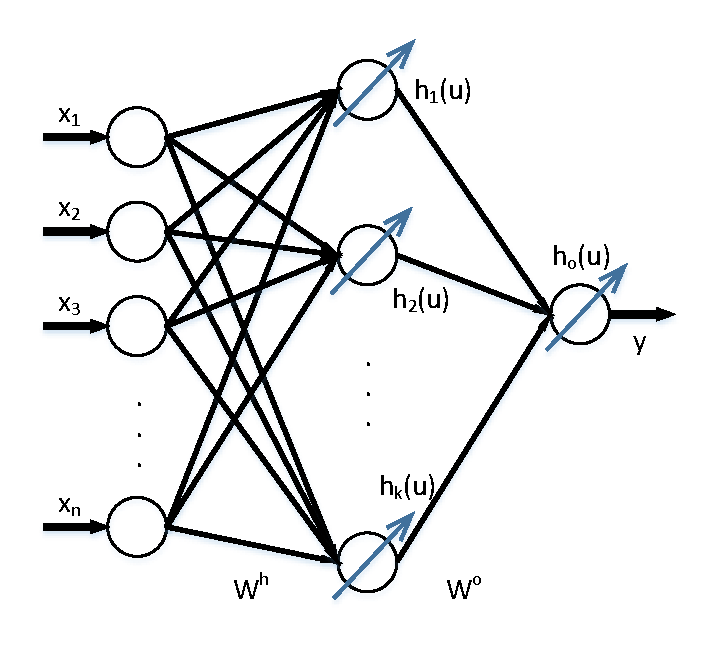
\includegraphics[width=0.5\textwidth]{fnn.pdf}
	\caption{一个单隐含层的人工神经网络,每一层的神经元个数分别是~$n,k,1$~,其中隐含层和输出层的神经元的~$k+1$~个激活函数是可调整的,即~$h_i(u) = 1 / (1 + e ^{-(\alpha_i u+\beta_i)}),~~i=1,2,\cdots,k,o$~。} \label{fig:fnn}
\end{figure}

首先,对网络进行前向计算,隐含层中每一个神经元的输入和输出分别为
\begin{align}
\bm{u} = \bm{W}^h ~ \bm{x},~~u_j = \sum_{i=1}^{n} W_{ji}^h ~ x_i,~~j=1,2,\cdots,k.\\
\bm{a} = h(\bm{u}),~~a_j = h_j(u_j),~~j=1,2,\cdots,k.
\end{align}
传至输出层,得到
\begin{align}
v = \bm{W}^o ~ \bm{a} = \sum_{j=1}^{k} W_j^o ~ a_j,~~y = h_o(v).
\end{align}
接着,定义目标函数,即平方误差项,(仅考虑一个输入样本)~,
\begin{align}
e = \frac{1}{2} (d- y)^2,
\end{align}
其中~$d$~表示期望输出值。为了使用梯度下降法,求出误差关于每一个权值的梯度值,
\begin{align}
\Delta W_j^o \varpropto  \frac{\partial e}{\partial W_j^o} &= \frac{\partial e}{\partial y} \frac{\partial y}{\partial v}\frac{\partial v}{\partial W_j^o} = -(d-y)~h_o'(v)~a_j,\\
\Delta W_{ji}^h \varpropto \frac{\partial e}{\partial W_{ji}^h} &= \frac{\partial e}{\partial y}\frac{\partial y}{\partial v}\frac{\partial v}{\partial a_j}\frac{\partial a_j}{\partial u_j}\frac{\partial u_j}{\partial W_{ji}^h} = -(d-y)~h'_o(v)~W_j^o~h_j'(u_j)~x_i,\\
h_o'(v) = \frac{\partial y}{\partial v} &= h_o(v)(1 - h_o(v)) \cdot \alpha_o = \alpha_o ~ y (1 - y), \\
h_j'(u_j) = \frac{\partial a_j}{\partial u_j} &= h_j(u_j)(1 - h_j(u_j)) \cdot \alpha_j = \alpha_j ~ a_j (1 - a_j), \\
&i=1,2,\cdots,n,~~j=1,2,\cdots,k. \nonumber
\end{align}
进一步写出每一个神经元的激活函数的参数训练时的改变量,
\begin{align}
\Delta \alpha_j & \varpropto \frac{1}{\alpha_j} + u_j (1 - 2 a_j),~~\Delta \beta_j \varpropto 1 - 2 a_j. \\
\Delta \alpha_o & \varpropto \frac{1}{\alpha_o} + v (1 - 2 y),~~\Delta \beta_o \varpropto 1 - 2 y.
\end{align}
我们的联合学习机制可以总结为以下几步:
\begin{enumerate}
	\item 初始化。选取随机值赋给权值~$\bm{W}^h$~和~$\bm{W}^o$~,并给每一个神经元的激活函数的参数~$\alpha,\beta$~给予初始值~$1,0$~,分别为几个可学习的参数设定合适的学习率。
	\item 前向传播。采用批量的训练数据传入神经网络进行前向计算,得到各个神经元的输入值~$\bm{u},\bm{v}$~和输出值~$\bm{a},\bm{y}$~,并最终计算输出神经元的平方误差项~$e$~。
	\item 权值更新。计算误差关于每一个权值的梯度~$\partial e / \partial \bm{W}$~,使用传统的梯度下降法更新网络中的权值~$\bm{W}^h,\bm{W}^o$~。
	\item 激活函数更新。使用前向计算得到的各个神经元的输入值~$\bm{u},\bm{v}$~和输出值~$\bm{a},\bm{y}$~,根据信息最大化的学习算法,更新隐含层和输出层的激活函数的参数~$\alpha,\beta$~。
	\item 停止或迭代。当训练结果收敛,即误差项~$e$~的变化量很小,或者达到预先设置的最大迭代次数时,停止训练。
\end{enumerate}

\section{实验}
本文的实验是对提出的人工神经网络训练方式进行测试,但是代码编写测试未完成,因为算法没有良好的收敛结果~(见图~\ref{fig:IMcompare})~,可能试算法实现过程有错误,有待调试,所以未能给出本算法的令人信服的结果。后续的工作作为我们的研究方向,有待一进步完善。
\begin{figure}[htbp]
	\centering
	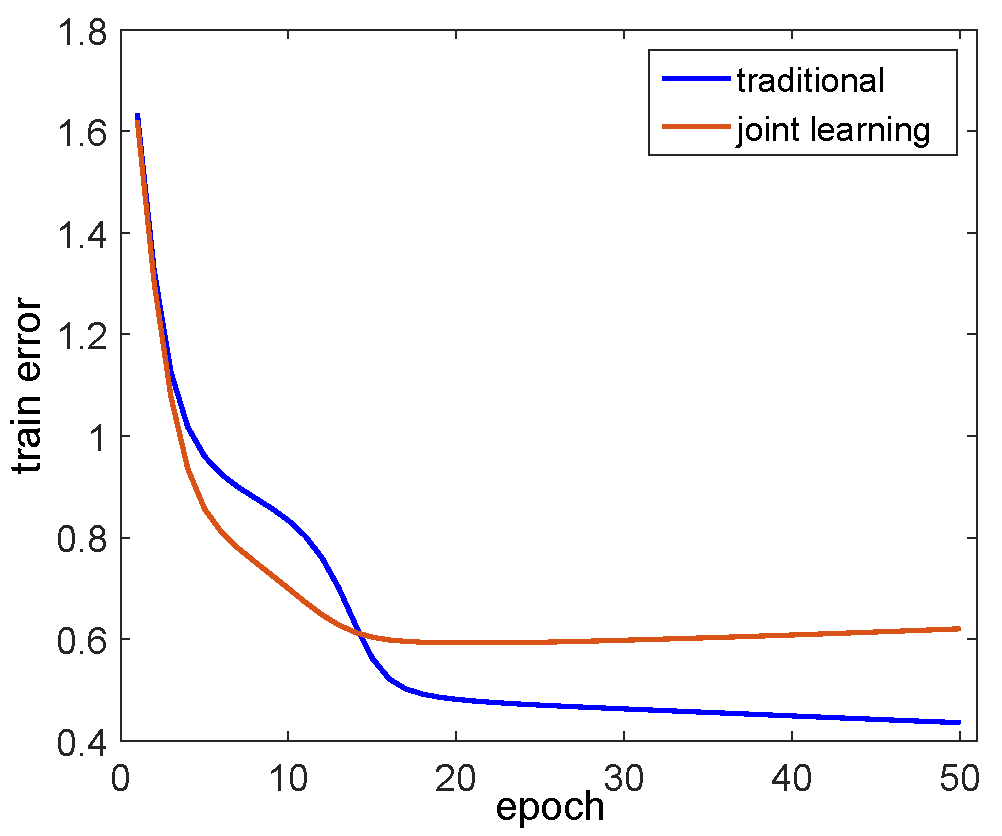
\includegraphics[width=0.5\textwidth]{IMcompare.pdf}
	\caption{联合学习与传统学习的比较结果。} \label{fig:IMcompare}
\end{figure}
\appendix
\section{Proof of Logistic Function} \label{appendix1}
在激活函数为~$y=1/(1+e^{-u})$~和~$u=ax+b$~情况下,已经得到~$\partial y / \partial x = ay(1-y)$~,那么可以计算
\begin{align}
\frac{\partial}{\partial a} \left( \frac{\partial y}{\partial x} \right) &= \frac{\partial}{\partial a} [ ay(1-y) ] \nonumber \\
&= y(1-y) + a \frac{\partial}{\partial a} (y - y^2) \nonumber \\
&= y(1-y) + a \left( \frac{\partial y}{\partial a} - 2y \frac{\partial y}{\partial a} \right) \nonumber \\
&= y(1-y) + a(1-2y)\frac{\partial y}{\partial u} \frac{\partial u}{\partial a} \nonumber \\
&= y(1-y) + a(1-2y) \cdot y(1-y) \cdot x \nonumber \\
&= y(1-y)[1+ax(1-2y)]. 
\end{align}
对偏置~$b$~考虑,
\begin{align}
\frac{\partial}{\partial b} \left( \frac{\partial y}{\partial x} \right) &= \frac{\partial}{\partial b} [ ay(1-y) ] \nonumber \\
&= a \left( \frac{\partial y}{\partial b} - 2y \frac{\partial y}{\partial b} \right) \nonumber \\
&= a(1-2y)\frac{\partial y}{\partial u} \frac{\partial u}{\partial b} \nonumber \\
&= a(1-2y) \cdot y(1-y) \cdot 1 \nonumber \\
&= a(1-2y)y(1-y). 
\end{align}

\section{Proof of Tanh Function} \label{appendix2}
在激活函数为~$y=\tanh(u)$~和~$u=ax+b$~情况下,已经得到
\begin{align}
\frac{\partial y}{\partial x} = \frac{\partial y}{\partial u} \frac{\partial u}{\partial x} = a(1-y^2),
\end{align}
,那么可以计算
\begin{align}
\frac{\partial}{\partial a} \left( \frac{\partial y}{\partial x} \right) &= \frac{\partial}{\partial a} [ a(1-y^2) ] \nonumber \\
&= 1-y^2 + a (-2y)\frac{\partial y}{\partial a} \nonumber \\
&= 1-y^2 + a (-2y) \frac{\partial y}{\partial u} \frac{\partial u}{\partial a} \nonumber \\
&= 1-y^2 - 2ay (1-y^2) x \nonumber \\
&= (1-y^2)(1 - 2axy). 
\end{align}
对偏置~$b$~考虑,
\begin{align}
\frac{\partial}{\partial b} \left( \frac{\partial y}{\partial x} \right) &= \frac{\partial}{\partial b} [ a(1-y^2) ] \nonumber \\
&= a(-2y)\frac{\partial y}{\partial u} \frac{\partial u}{\partial b} \nonumber \\
&= -2ay(1-y^2).
\end{align}
此时~tanh~函数的学习规则得出,
\begin{align}
\Delta a \varpropto \frac{\partial H}{\partial a} &= \left( \frac{\partial y}{\partial x} \right)^{-1} \frac{\partial}{\partial a} \left( \frac{\partial y}{\partial x} \right) = \frac{1}{a} - 2xy. \\
\Delta b \varpropto \frac{\partial H}{\partial b} &= \left( \frac{\partial y}{\partial x} \right)^{-1} \frac{\partial}{\partial b} \left( \frac{\partial y}{\partial x} \right) = -2y.
\end{align}

\bibliographystyle{ieeetr}
\bibliography{mybibliography}

\end{document}

